\documentclass[a4paper,12pt]{report}
\usepackage[toc,page]{appendix}
\usepackage{amsmath}
\usepackage{float}
\usepackage{graphicx}
\usepackage{subfig}
\usepackage{amssymb}
\usepackage{geometry}
\usepackage{array}
\usepackage{tcolorbox}
\usepackage[normalem]{ulem}

\usepackage{setspace}
 \geometry{
 a4paper,
 total={170mm,257mm},
 left=20mm,
 top=20mm,
 }
\usepackage{tikz}
\usepackage{pgfplots}
\usetikzlibrary{shapes, arrows.meta, decorations.pathreplacing, positioning, petri, fit, calc}
\tikzstyle{startstop} = [circle, minimum size=1cm ,text centered, draw=black]
\tikzstyle{neuron} = [circle, minimum size=1cm ,text centered, draw=red, fill=gray!30]
\tikzstyle{neuronEll} = [ellipse, minimum size=1cm ,text centered, text width=2cm, draw=red, fill=gray!30]
\tikzstyle{process} = [rectangle, minimum width=2cm, minimum height=0.5cm, text centered, text width=3cm, draw=black, fill=blue!30]
\tikzstyle{detail} = [rectangle, minimum width=1.5cm, minimum height=0.5cm, text justified, text width=2.6cm, fill=white!30]
\tikzstyle{smalldetail} = [rectangle, minimum width=2cm, minimum height=1cm, text centered, text width=2cm]
\tikzstyle{largedetail} = [rectangle, minimum width=3cm, minimum height=1cm, text centered, text width=4cm, fill=white!30]
\tikzstyle{box} = [rectangle, minimum width=5cm, minimum height=9cm, text centered, text width=4cm, draw=black, fill=white!30]

\usepackage[utf8]{inputenc}

% Default fixed font does not support bold face
\DeclareFixedFont{\ttb}{T1}{txtt}{bx}{n}{10} % for bold
\DeclareFixedFont{\ttm}{T1}{txtt}{m}{n}{10}  % for normal

% Custom colors
\usepackage{color}
\definecolor{deepblue}{rgb}{0,0,0.5}
\definecolor{deepred}{rgb}{0.6,0,0}
\definecolor{deepgreen}{rgb}{0,0.5,0}

\usepackage{listings}

% Python style for highlighting
\newcommand\pythonstyle{\lstset{
language=Python,
basicstyle=\ttm,
otherkeywords={self},             % Add keywords here
keywordstyle=\ttb\color{deepblue},
emph={MyClass,__init__},          % Custom highlighting
emphstyle=\ttb\color{deepred},    % Custom highlighting style
stringstyle=\color{deepgreen},
frame=tb,                         % Any extra options here
showstringspaces=false            % 
}}


% Python environment
\lstnewenvironment{python}[1][]
{
\pythonstyle
\lstset{#1}
}
{}

% Python for external files
\newcommand\pythonexternal[2][]{{
\pythonstyle
\lstinputlisting[#1]{#2}}}

% Python for inline
\newcommand\pythoninline[1]{{\pythonstyle\lstinline!#1!}}


\begin{document}
\tableofcontents

\title{Debugging a Learning Algorithm}
\maketitle
\part{Week 6}
\section{Machine Learning Diagnostic}
It is important to run tests to gain insight of what is/isn't working with a learning algorithm.

\subsection{Evaluating a hypothesis }
\textbf{Because a hypothesis has low training error does not mean the hypothesis is best} (could be overfitting).
One approach to test an hypothesis, is to split the dataset into 2 sub-sets after shuffling (mixing)  the data:
\begin{itemize}
\item Training set ($\approx$70\% of the entire dataset)
\item Test set ($\approx$30\%)
\end{itemize}

\begin{itemize}
\item Training/Testing procedure for \textbf{linear regression}:
\begin{itemize}
	\item Learn parameter $\theta$ from training data (minimum training error $J(\theta)$)
	\item Compute test set error using $\theta$ values obtained the training set:
	\begin{align}
	J_{test} (\theta) = \frac{1}{2 m_{test}} \sum_{i=1} ^{m_{test}} \left(h_{\theta}(x_{test} ^{(i)}) - y_{test} ^{(i)} \right)^2
	\end{align}
\end{itemize}
\end{itemize}


\begin{itemize}
\item Training/Testing procedure for \textbf{logistic regression}:
\begin{itemize}
	\item Learn parameter $\theta$ from training data (minimum training error $J(\theta)$)
	\item Compute test set error using $\theta$ values obtained the training set:
	\begin{align}
	J_{test} (\theta) = \frac{-1}{2 m_{test}} \sum_{i=1} ^{m_{test}} y_{test} ^{(i)} \mathrm{log}(h_{\theta}(x_{test}^{(i)})) + (1-y_{test} ^{(i)}) \mathrm{log}(1-h_{\theta}(x_{test}^{(i)}))
	\end{align}
	\item Alternative: misclassification error ("0/1 misclassification")
	\begin{align*}
	\mathrm{err}(h_{\theta}(x), y)=
	\begin{cases}
		1  & \mathrm{\ if\ } h_{\theta}(x) \geq 0.5 \mathrm{\ and \ }y=0\\
		   & \mathrm{\ or if\ } h_{\theta}(x) < 0.5 \mathrm{\ and \ }y=1\\
		0  & \mathrm{\ otherwise \ (hypothesis \ classify \ the \ example\  correctly } \\
	\end{cases}
	\end{align*} 
	\begin{align}
	\mathrm{testErr}=\frac{1}{m_{test}} \sum_{i=1} ^{m_{test}} \mathrm{err}(h_{\theta}(x_{test} ^{(i)}, y_{test} ^{(i)})
	\end{align}
	This is the fraction of the examples in the \textbf{test set} that the hypothesis labeled.
\end{itemize}
\end{itemize}

\subsection{Model selection and training/validation/test}
\begin{itemize}
\item we want to decide on a model for the hypothesis ($d$ is the degree of polynomial):
\begin{enumerate}
\item $h_{\theta}(x) = \theta_0 + \theta_1 x$  ($d$=1)
\item $h_{\theta}(x) = \theta_0 + \theta_1 x + \theta_2 x^2$  ($d$=2)
\item $h_{\theta}(x) = \theta_0 + \theta_1 x + \theta_2 x^2 + \theta_3 x^3$  ($d$=3)\\ 
.......... \\
.........
\item $h_{\theta}(x) = \theta_0 + \theta_1 x + \theta_2 x^2 + ... +  \theta_{10} x^{10}$  ($d$=10)
\end{enumerate}
\end{itemize}

One option is to fit all the models to the train data and then compute $J_{test}(\theta^{(d)})$, and select the model giving the lowest test set error.
\begin{enumerate}
\item $h_{\theta}(x) = \theta_0 + \theta_1 x$  ($d$=1) $\rightarrow$ $\theta^{(1)}$  $\rightarrow$ $J_{test}(\theta^{(1)})$
\item $h_{\theta}(x) = \theta_0 + \theta_1 x + \theta_2 x^2$  ($d$=2) $\rightarrow$ $\theta^{(2)}$  $\rightarrow$ $J_{test}(\theta^{(2)})$
\item $h_{\theta}(x) = \theta_0 + \theta_1 x + \theta_2 x^2 + \theta_3 x^3$  ($d$=3) $\rightarrow$ $\theta^{(3)}$  $\rightarrow$ $J_{test}(\theta^{(3)})$\\ 
.......... \\
.........
\item $h_{\theta}(x) = \theta_0 + \theta_1 x + \theta_2 x^2 + ... +  \theta_{10} x^{10}$  ($d$=10) $\rightarrow$ $\theta^{(10)}$  $\rightarrow$  $J_{test}(\theta^{(10)})$
\end{enumerate}

How well the model generalize to new examples, cannot be determined by selecting the model with the lowest $J_{test}(\theta^{(d)})$. Indeed, if we develop new features by examining the test set, then we may end up choosing features that work well specifically for the test set. So, $J_{test}(\theta)$ is no longer a good estimate of how well we generalize to new examples.\\

\begin{itemize}
\item In fact a more robust approach is to split the dataset into 3 parts:
\end{itemize}
\begin{enumerate}
\item Training set ($\approx$60\% of dataset) with training error: \\
\begin{align}
J_{train}(\theta) = \frac{1}{2m_{train}} \sum_{i=1} ^{m_{train}} (h_{\theta} (x_{train} ^{(i)}) -y_{train} ^{(i)})^2
\end{align}
\item Cross validation (CV) or Validation set ($\approx$20\%) with cross validation error: \\
\begin{align}
J_{cv}(\theta) = \frac{1}{2m_{cv}} \sum_{i=1} ^{m_{cv}} (h_{\theta} (x_{cv} ^{(i)}) -y_{cv} ^{(i)})^2
\end{align}
\item Test set ($\approx$20\%) with test error: 
\begin{align}
J_{test}(\theta) = \frac{1}{2m_{test}} \sum_{i=1} ^{m_{test}} (h_{\theta} (x_{test} ^{(i)} -y_{test} ^{(i)})^2
\end{align}
\end{enumerate}

When faced with a model selection problem, we will use Cross Validation error:
\begin{enumerate}
\item $h_{\theta}(x) = \theta_0 + \theta_1 x$  ($d$=1) $\rightarrow$ $\theta^{(1)}$  $\rightarrow$ $J_{cv}(\theta^{(1)})$
\item $h_{\theta}(x) = \theta_0 + \theta_1 x + \theta_2 x^2$  ($d$=2) $\rightarrow$ $\theta^{(2)}$  $\rightarrow$ $J_{cv}(\theta^{(2)})$
\item $h_{\theta}(x) = \theta_0 + \theta_1 x + \theta_2 x^2 + \theta_3 x^3$  ($d$=3) $\rightarrow$ $\theta^{(3)}$  $\rightarrow$ $J_{cv}(\theta^{(3)})$\\ 
.......... \\
.........
\item $h_{\theta}(x) = \theta_0 + \theta_1 x + \theta_2 x^2 + ... +  \theta_{10} x^{10}$  ($d$=10) $\rightarrow$ $\theta^{(10)}$  $\rightarrow$  $J_{cv}(\theta^{(10)})$
\end{enumerate}
We select the model resulting in the lowest Cross validation error $J_{cv}(\theta^{(d)})$, and use it on the test set to check the generalization of the model.


\section{Diagnosing Bias vs. Variance}
\begin{itemize}
\item \textbf{Definition}:
\begin{itemize}
\item High Bias = underfit
\item High Variance = overfit
\end{itemize}
\end{itemize}

\subsection{Choice of model}
Let's consider the problem of choosing the polynomial degree ($d$) of the model:
\begin{figure}[H]
	\centering
        \includegraphics[totalheight=5 cm]{polydeg.png}
\end{figure}
If the algorithm suffers from:
\begin{itemize}
\item High Bias (underfit): $J_{train}(\theta) \approx J_{cv}(\theta)$, both high
\item Variance (overfit): $J_{train}(\theta)$ is low and $J_{cv}(\theta) >> J_{train}(\theta)$
\end{itemize}
\subsection{Regularization ($\lambda$) and Bias/Variance }
Increasing regularization helps to fix High variance (overfitting).
\begin{itemize}
\item Model:
\begin{align}
h_{\theta}(x) = \theta_0 + \theta_1 x + \theta_2 x^2 + \theta_3 x^3 + \theta_4 x^4 
\end{align}
\begin{align}
h_{\theta}(x) = \frac{1}{2m} \sum_{i=1} ^{m} (h_{\theta}(x^{(i)}-y^{(i)})^2 + \frac{\lambda}{2m} \sum_{j=1} ^m \theta_j ^2
\end{align}
\end{itemize}

\begin{itemize}
\item Choosing the regularization parameter $\lambda$:
\begin{itemize}
\item (1) try $\lambda=0 \Rightarrow$ ${\mathrm{min}}_{\theta} J_{test}(\theta^{(1)}) \rightarrow \theta^{(1)} \Rightarrow J_{cv}(\theta^{(1)})$
\item (2) try $\lambda=0.01$ $\Rightarrow$ ${\mathrm{min}}_{\theta} J_{test}(\theta^{(2)}) \rightarrow \theta^{(2)} \Rightarrow J_{cv}(\theta^{(2)})$
\item (3) try $\lambda=0.02$ $\Rightarrow$ ${\mathrm{min}}_{\theta} J_{test}(\theta^{(3)}) \rightarrow \theta^{(3)} \Rightarrow J_{cv}(\theta^{(3)})$
\item (4) try $\lambda=0.04$ $\Rightarrow$ ${\mathrm{min}}_{\theta} J_{test}(\theta^{(4)}) \rightarrow \theta^{(4)} \Rightarrow J_{cv}(\theta^{(4)})$ \\
...\\
...\\
...\\
\item (12) try $\lambda=10$ $\Rightarrow$ ${\mathrm{min}}_{\theta} J_{test}(\theta^{(10)}) \Rightarrow \theta^{(10)} \rightarrow J_{cv}(\theta^{(10)})$
\end{itemize}
\end{itemize}
Pick $\lambda$ with lowest $J_{cv}(\theta^{(\lambda)})$ and compute $J_{test}(\theta^{(\lambda)})$
\begin{figure}[H]
	\centering
        \includegraphics[totalheight=5 cm]{regularization.png}
\end{figure}

\subsection{Learning curves: training size}
\begin{itemize}
\item case of High Bias
\end{itemize}
\begin{figure}[H]
\begin{center}$
\begin{array}[m]{r|l}
        \includegraphics[totalheight=5 cm]{HiBias_learningCurve.png}
& 
\begin{array}[b]{l}
\textbf{If \ algorithm \ suffers \ from \  High \ Bias:} \\
\mathrm{1) \ residual \ error \ }J_{train}(\theta) \mathrm{\ and \ }J_{cv}(\theta) \mathrm{\ is \ high} \\
\mathrm{2)\ } J_{train}(\theta) \approx J_{cv}(\theta) \\
\mathrm{3)\ Increasing\  Nbr\  of\  training\  data\  will\  not\  help\  by\  itself}\\
\end{array}
\end{array}$
\end{center}
\end{figure}

\begin{itemize}
\item Case of High Variance (for example: use of a high order polynomial hypothesis)
\end{itemize}
\begin{figure}[H]
\begin{center}$
\begin{array}[m]{r|l}
        \includegraphics[totalheight=5 cm]{HiVariance_learningCurve.png}
& 
\begin{array}[b]{l}
\textbf{If \ algorithm\  suffers\  from\  High\  variance\  :}\\
\mathrm{1) \ residual\  error\  of\ } J_{train}(\theta) \mathrm{\ is\  low} \\
\mathrm{2)\ }J_{cv}(\theta) >> J_{train}(\theta) \\
\mathrm{3)\ } \mathrm{Increasing \  Nbr\  of\  training\  data\  is\  likely\  to\  help} \\
\end{array}
\end{array}$
\end{center}
\end{figure}

\section{steps to debug a learning algorithm}
Suppose we have implemented regularized linear regression to predict housing prices. However, when you test your hypothesis on a new set of houses, you find that it makes unacceptably large errors in its prediction.
\begin{itemize}
\item Get more training examples $\rightarrow$ to fix high variance
\item try smaller sets of features $\rightarrow$ to fix high variance
\item try getting additional features $\rightarrow$ to fix high bias
\item try adding polynomial features $\rightarrow$ to fix high bias
\item decrease $\lambda$ $\rightarrow$ to fix high bias
\item increase $\lambda$ $\rightarrow$ to fix high variance
\end{itemize}

\section{Neural Network}
\begin{figure}[H]
\begin{center}$
\begin{array}[b]{l|c|l}
\mathrm{small \ NN \ with \ fewer \ parameters} & \mathrm{Large \ Network} & \mathrm{Large \ Network}\\
\mathrm{more\  prone \ to\  underfitting} & \mathrm{more \ prone\  to\  overfitting} & \mathrm{more \ prone\  to\  overfitting}\\
\resizebox {1.5in} {!} {
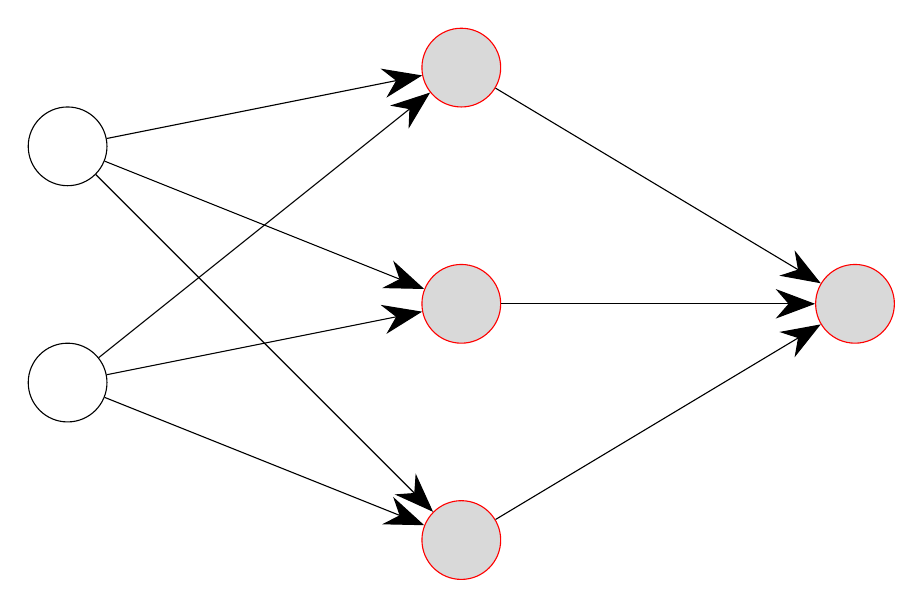
\begin{tikzpicture}[node distance=3cm]
\node (x0) [startstop] {};
\node (x1) [startstop, below of=x0, xshift=0cm, yshift=0cm] {};
\node (a01) [neuron, below of=x0, xshift=5cm, yshift=4cm] {};
\node (a11) [neuron, below of=a01, xshift=0cm, yshift=0cm] {};
\node (a12) [neuron, below of=a11, xshift=0cm, yshift=0cm] {};
\node (output) [neuron, below of=a01, xshift=5cm, yshift=0cm] {};
\draw [-{Stealth[length=5mm]}] (x0) -- (a01);
\draw [-{Stealth[length=5mm]}] (x0) -- (a11);
\draw [-{Stealth[length=5mm]}](x0) -- (a12);
\draw [-{Stealth[length=5mm]}] (x1) -- (a01);
\draw [-{Stealth[length=5mm]}] (x1) -- (a11);
\draw [-{Stealth[length=5mm]}] (x1) -- (a12);
\draw [-{Stealth[length=5mm]}] (a01) -- (output);
\draw [-{Stealth[length=5mm]}] (a11) -- (output);
\draw [-{Stealth[length=5mm]}] (a12) -- (output);
\end{tikzpicture} }
& 
\resizebox {1.5in} {!} {
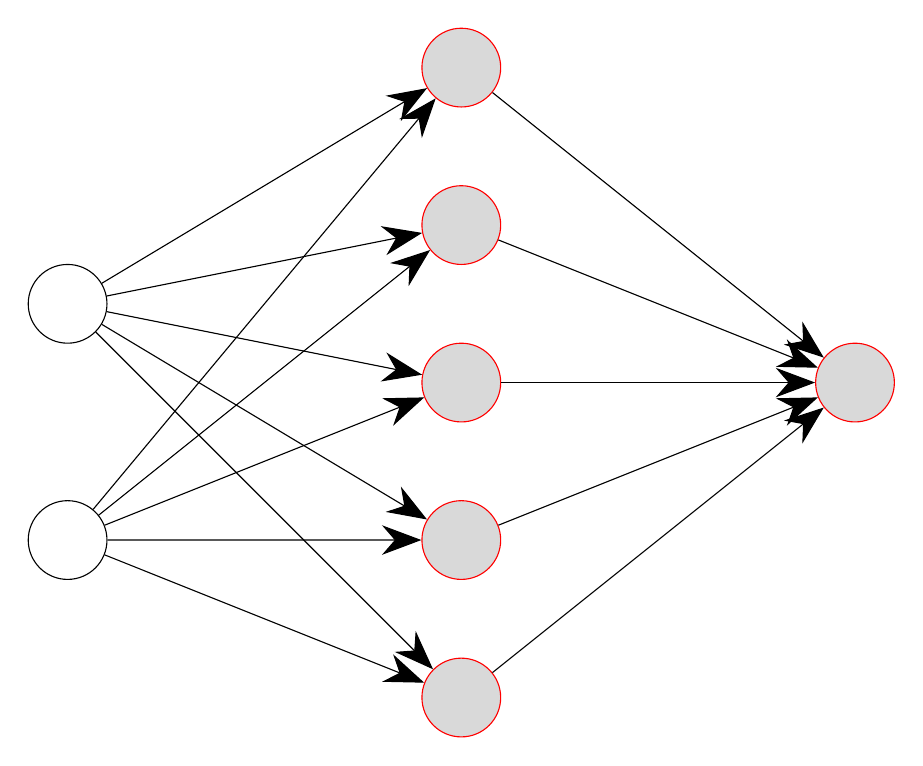
\begin{tikzpicture}[node distance=3cm]
\node (x0) [startstop] {};
\node (x1) [startstop, below of=x0, xshift=0cm, yshift=0cm] {};
\node (a01) [neuron, below of=x0, xshift=5cm, yshift=6cm] {};
\node (a11) [neuron, below of=a01, xshift=0cm, yshift=1cm] {};
\node (a21) [neuron, below of=a11, xshift=0cm, yshift=1cm] {};
\node (a31) [neuron, below of=a21, xshift=0cm, yshift=1cm] {};
\node (a41) [neuron, below of=a31, xshift=0cm, yshift=1cm] {};
\node (output) [neuron, below of=a21, xshift=5cm, yshift=3cm] {};
\draw [-{Stealth[length=5mm]}] (x0) -- (a01);
\draw [-{Stealth[length=5mm]}] (x0) -- (a11);
\draw [-{Stealth[length=5mm]}] (x0) -- (a21);
\draw [-{Stealth[length=5mm]}] (x0) -- (a31);
\draw [-{Stealth[length=5mm]}] (x0) -- (a41);
\draw [-{Stealth[length=5mm]}](x1) -- (a01);
\draw [-{Stealth[length=5mm]}](x1) -- (a11);
\draw [-{Stealth[length=5mm]}](x1) -- (a21);
\draw [-{Stealth[length=5mm]}] (x1) -- (a31);
\draw [-{Stealth[length=5mm]}] (x1) -- (a41);
\draw [-{Stealth[length=5mm]}](a01) -- (output);
\draw [-{Stealth[length=5mm]}](a11) -- (output);
\draw [-{Stealth[length=5mm]}](a21) -- (output);
\draw [-{Stealth[length=5mm]}] (a31) -- (output);
\draw [-{Stealth[length=5mm]}] (a41) -- (output);
\end{tikzpicture} } 
&
\resizebox {1.5in} {!} {
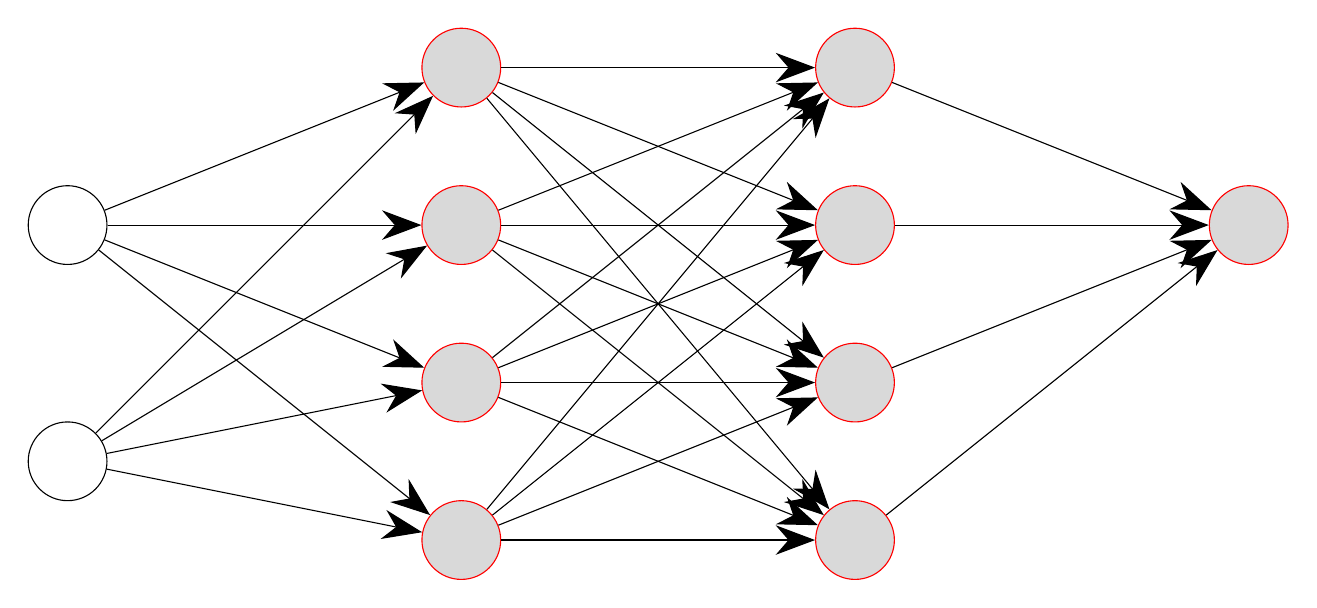
\begin{tikzpicture}[node distance=3cm]
\node (x0) [startstop] {};
\node (x1) [startstop, below of=x0, xshift=0cm, yshift=0cm] {};
\node (a01) [neuron, below of=x0, xshift=5cm, yshift=5cm] {};
\node (a11) [neuron, below of=a01, xshift=0cm, yshift=1cm] {};
\node (a21) [neuron, below of=a11, xshift=0cm, yshift=1cm] {};
\node (a31) [neuron, below of=a21, xshift=0cm, yshift=1cm] {};
\node (a02) [neuron, below of=x0, xshift=10cm, yshift=5cm] {};
\node (a12) [neuron, below of=a02, xshift=0cm, yshift=1cm] {};
\node (a22) [neuron, below of=a12, xshift=0cm, yshift=1cm] {};
\node (a32) [neuron, below of=a22, xshift=0cm, yshift=1cm] {};
\node (output) [neuron, below of=x0, xshift=15cm, yshift=3cm] {};
\draw [-{Stealth[length=5mm]}] (x0) -- (a01);
\draw [-{Stealth[length=5mm]}] (x0) -- (a11);
\draw [-{Stealth[length=5mm]}] (x0) -- (a21);
\draw [-{Stealth[length=5mm]}] (x0) -- (a31);
\draw [-{Stealth[length=5mm]}](x1) -- (a01);
\draw [-{Stealth[length=5mm]}](x1) -- (a11);
\draw [-{Stealth[length=5mm]}](x1) -- (a21);
\draw [-{Stealth[length=5mm]}] (x1) -- (a31);
\draw [-{Stealth[length=5mm]}] (a01) -- (a02);
\draw [-{Stealth[length=5mm]}] (a11) -- (a02);
\draw [-{Stealth[length=5mm]}] (a21) -- (a02);
\draw [-{Stealth[length=5mm]}] (a31) -- (a02);
\draw [-{Stealth[length=5mm]}] (a01) -- (a12);
\draw [-{Stealth[length=5mm]}] (a11) -- (a12);
\draw [-{Stealth[length=5mm]}] (a21) -- (a12);
\draw [-{Stealth[length=5mm]}] (a31) -- (a12);
\draw [-{Stealth[length=5mm]}] (a01) -- (a22);
\draw [-{Stealth[length=5mm]}] (a11) -- (a22);
\draw [-{Stealth[length=5mm]}] (a21) -- (a22);
\draw [-{Stealth[length=5mm]}] (a31) -- (a22);
\draw [-{Stealth[length=5mm]}] (a01) -- (a32);
\draw [-{Stealth[length=5mm]}] (a11) -- (a32);
\draw [-{Stealth[length=5mm]}] (a21) -- (a32);
\draw [-{Stealth[length=5mm]}] (a31) -- (a32);
\draw [-{Stealth[length=5mm]}](a02) -- (output);
\draw [-{Stealth[length=5mm]}](a12) -- (output);
\draw [-{Stealth[length=5mm]}](a22) -- (output);
\draw [-{Stealth[length=5mm]}] (a32) -- (output);
\end{tikzpicture} } \\
& \mathrm{more \ hidden \ layer\  units} & \mathrm{more \ hidden \ layers} \\
& \mathrm{Use \ regularization } & \mathrm{Use \ regularization} \\
& \mathrm{to \ adress \ overfitting} & \mathrm{to \ adress \ overfitting}
\end{array}$
\end{center}
\end{figure}

Using a larger NN with regularization is often more effective than a small NN.
In order to determine what architecture is best (large Nbr of hidden units or larger Nbr of hidden layers), use Train/CV/Test split and evaluate the architecture with CV error ($J_{cv}(\theta))$


\section{Error Analysis}
When  developing an algorithm, it is advised to :
\begin{itemize}
\item start with a simple model and check it with cross validation data
\item plot learning curves to decide if more data, more features... are likely to help
\item Error analysis: 
	\begin{itemize}
		\item manually examine the examples in cross validation set where the algorithm made errors on.
		\item classify the errors and prioritize on the error to tackle \\
		For example, in spams classifier if among the misclassified emails, one finds:
	
		\begin{table}[!htbp]
		\centering
		\begin{tabular}[H]{|c|c|}
		  \hline \\
		  pharma & 12 examples \\
			\hline
			replica/fake & 4 \\
			\hline
			steal pwds & 53 \\
			\hline
			other & 31 \\
			\hline
		\end{tabular}
		\end{table}
		That suggests that emails 'steal pwds' is the category that degrades the algorithm performance . 
	\end{itemize}
\end{itemize}

\section{Error metrics for skewed classes}
\begin{itemize}
\item Definition: case of \textbf{skewed classes} occur when in the dataset there is much more examples of one class over the class.
\end{itemize}
For skewed classes, classification accuracy is not a good metric for the performance of the algorithm. It is better to use \textbf{Precision}/ \textbf{Recall} parameters:
\begin{table}[!htbp]
\centering
		\begin{tabular}[H]{|c|c|c|}
		  \hline
		 Predicted class & \multicolumn{2}{c}{Actual class} \\
		\hline
			& 1 & 0 \\
			\hline
			 1 & True Positive & False Positive \\
			\hline
			0 & False Negative & True Negative \\
			\hline
		\end{tabular}
\end{table}
\begin{align}
\begin{split}
P &= \frac{\mathrm{\# \ True\  Positive}}{\mathrm{\# \ Predicted\  Positive}} = \frac{\mathrm{\# \ True\  Positive}}{\mathrm{True \ Positive \ +\ False\  Positive}}\\
& \\
R &= \frac{\mathrm{\# \ True\  Positive}}{\mathrm{\# \ actual\  Positive}} = \frac{\mathrm{\# \ True\  Positive}}{\mathrm{True \ Positive \ +\ False\  Negative}}\\
\end{split}
\end{align}
We typically target High recall and High Precision for a performing algorithm.\\
\begin{itemize}
\item In the case of skewed classes, the convention is to label the rare class as $y=1$
\end{itemize}

\begin{itemize}
\item \textbf{Trade off between Precision/Recalls}.\\
\begin{itemize}
\item Increase the precision (P) by increasing the threshold:
\begin{itemize}
\item Predict 1 if $h_{\theta}(x) > $ \sout{0.5} \ \ 0.7
\item Predict 1 if $h_{\theta}(x) < $ \sout{0.5} \ \ 0.7
\end{itemize}
Decrease threshold $\Longrightarrow$ Higher Precision / Lower Recall.
\end{itemize}
\begin{itemize}
\item Increase the Recall (R) by decreasing the threshold (avoid 'False negative')
\begin{itemize}
\item Predict 1 if $h_{\theta}(x) \geq $ \sout{0.5} \ \ 0.3
\item Predict 1 if $h_{\theta}(x) < $ \sout{0.5} \ \ 0.3
\end{itemize}
Decrease threshold $\Longrightarrow$ Higher Recall / Lower Precision.
\end{itemize}
More generally, we want to predict 1 if $h_{\theta}(x) < threshold$, depending if we target higher recall or higher precision.
\end{itemize}
\begin{figure}[H]
\centering
        \includegraphics[totalheight=4 cm]{recallprec.png}
						\caption{
								\label{housingData} The precision/recall curve can have different shapes}
\end{figure}
\begin{itemize}
\item Optimum Precision/Recall is determined with $F_1$ score (target = Higher $F_1$):
\begin{align}
F_1 = 2 \frac{P R}{P + R}
\end{align}
There are other expressions for $F_1$ score.\
\end{itemize}
\end{document}